\section{Erhebung Ist-Zustandes}
\label{kap:istzustand}
\subsection{Problemstellung}
Der Business Transformation Tracker (BTT) ist ein essentieller Bestandteil der adesso active transformation. Er soll dazu dienen alle im Transformationsprojekt betrachteten und im alten SAP-System abgebildeten Geschäftsprozesse inkl. ihrer Subprozesse und Prozessschritte zu erfassen, um sie entlang der Transformation zu begleiten und übersichtlich den Fortschritt der Transformation zu dokumentieren. Dadurch möchte man erreichen, dass die betrachteten Geschäftsprozesse und Prozesschritte stets unter den selben Gesichtspunkten betrachtet und bewertet werden, wodurch zum einen die Transformation der Geschäftsrozesse hinterher wiedergegeben und zurückverfolgt werden kann und zum anderen für die Projektleitung stets der aktuelle Fortschritt eingeholt werden kann. Auch soll der BTT als Verzeichnis für alle den Prozess betreffende Informationen, wie z.B. den verwendeten SAP-Transaktionscodes oder der Verortung der Beschreibung im Fachkonzept, aber auch als Checkliste für vorzunehmende Maßnahmen, wie zum Beispiel der Aktualisierung des Benutzerhandbuchs oder der Beschreibung des Geschäftsprozesses im Fachkonzept, dienen. Diese zu bewertenen Kriterien werden zu Beginn eines Projektes durch den (Teil-)Projektleiter, in Zusammenarbeit mit dem Kunden, definiert und unterscheiden sich von Projekt zu Projekt, aber auch innerhalb eines Projekts, von Teilprojekt zu Teilprojekt. Der BTT soll logisch in die verschiedenen Projektphasen der adesso active transformation unterteilbar sein und soll dadurch auch den Projektplan in seinen Grundzügen wiedergeben können.


\subsection{Beschreibung Ist-Zustand}
Zum jetzigen Zeitpunkt exisitiert eine Implementierung des Business Transformation Trackers in Form einer Spreadsheet-Vorlage. Diese kommt bereits in einigen adesso active transformation -Projekten zum Einsatz und unterstützt dabei bereits heute die Projektmitarbeiter.\\ Aufgebaut und bearbeitet wird das Dokument mit Hilfe des Programms Microsoft Excel, das durch seine globale Verbreitung als Standardsoftware für Tabellenkalkulation\footcite[Vgl.][]{wiki-excel} allgemein bekannt ist und bei der adesso orange AG sowie ihren Kunden zum Einsatz kommt.\\
\begin{figure}[h!]
    \centering
    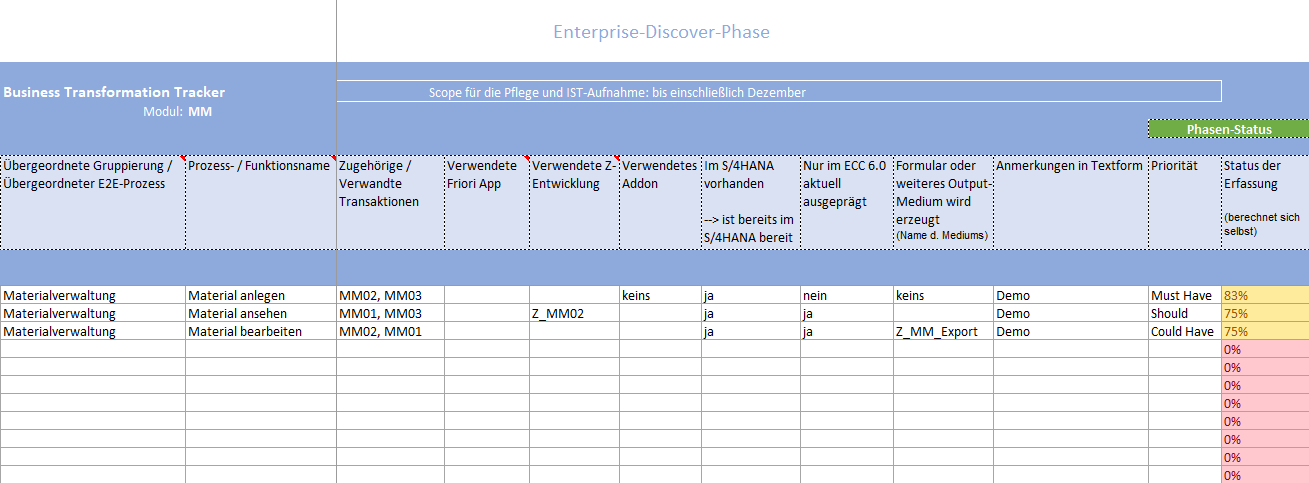
\includegraphics[scale=0.45]{./Bilder/BTT-Ist.png}
    \caption[Istzustand BTT]{Screenshot des Spreadsheets (Quelle: adesso orange AG)}
\end{figure}
\\Der Aufbau des Spreadsheets gliedert sich in die Spalten- und Zeilendimension: Im linken Kopfbereich der Tabelle sind die Basisinformationen des Dokuments enthalten, wie z.B. das zugehörige Projekt und das betrachtete SAP-Modul. Die Definition der betrachteten Transformationskriterien erfolgt auf Ebene der Tabellenspalten. Dabei ist je Kriterium eine Spalte vorgesehen, das im Kopfbereich der Tabelle definiert ist. Über der Zeile mit der Definition der Kritererien werden mehrere dieser logisch zu einer Projektphase zusammengefasst. Auf der Ebene der Tabellenzeilen werden die einzelnen Prozesse und die dazugehörigen Prozesschritte, beginnend unterhalb des Tabellenkopfs, nacheinander aufgeführt, sodass die betrachteten Prozesse vollständig in der Tabelle abgebildet werden. Danach erfolgt in jeder angelegten Tabellenzeile die Ausprägung der vorher definierten Kriterien. Dabei wird so vorgegangen, dass auf der linken Seite mit dem ersten Kriterium begonnen wird und stetig von links-nach-rechts ein Kriterium nach dem anderen ausgeprägt wird, bis schließlich die komplette Projektphase befüllt ist. Zum Ende einer jeden Phasen ist ein Fortschrittsgrad implementiert, der sich pro Zeile aus der Anzahl der ausgefüllten Zellen, bzw. Kriterien ergibt. Es ist vorgesehen in der Tabelle alle betrachteten Projektphasen mit ihren jeweiligen Kriterien nebeneinander visuell abzubilden und durch die Gesamtheit des Tabellenblattes einen chronologischen Ablauf der Transformation eines Prozesschrittes zu erzeugen.\\Das Befüllen der Tabelle erstreckt sich in der Regel über den gesamten Projektzeitraum, was eine Zeit von mehreren Monaten bedeuten kann. Die Speicherung des BTT-Spreadsheets erfolgt zumeist lokal auf den Computern der Mitarbeiter, oder online in der vom Unternehmen genutzten Cloud-Plattform, \glqq{}Microsoft OneDrive\grqq{}. Teilweise kommt es auch vor, dass die Dokumente in der IT-Infrastruktur des Kunden abgelegt werden, da dies entweder aus Governance- bzw. Compliance-Vorgaben vorgegeben ist, oder die Projektmitarbeiter des Kunden ebenfalls Zugriff benötigen um mit den Dokumenten zu arbeiten.


\subsection{Bewertung der aktuellen Umsetzung}
%Quellen fehlen noch
Die aktuelle Form des BTT bietet in seiner jetzigen Umsetzung als Spreadsheet einige Vor- und Nachteile die im Folgenden genauer beleuchtet und dargestellt werden sollen. Die Umsetzung in Microsoft Excel ermöglicht eine einfache Bearbeitung durch die Mitarbeiter. Dazu sind keine speziellen IT- bzw. Programmierkenntnisse notwendig, da die Bedienung von Microsoft Office und somit auch des darin enthaltenen Microsoft Excel zu den Einstellungskriterien vieler Unternehmen gehört. Deshalb sollte somit fast jeder Mitarbeiter über die Fähigkeit verfügen, bspw. ein neues Kriterium durch eine zusätzliche Spalte hinzuzufügen. Dadurch ist es auch sehr einfach für die Mitarbeiter, auftretene Fehler, wie z.B. falsche Zellformeln oder fehlerhafte Darstellungen selbst mit wenigen Handgriffen zu beheben, ohne höhere Programmierkenntnisse besitzen zu müssen. Ebenfalls ist die generelle Arbeit mit Excel mit keinen großen Hürden verbunden, solange der Benutzer über einen Computer mit dem installierten Programm verfügt. Eine Internetverbindung ist dazu in der Regel, bei lokaler Verfügbarkeit der Datei, nicht notwendig, wodurch auch mobiles Arbeiten, z.B. aus der Bahn, möglich ist.\\Bei Microsoft Excel handelt es sich um weitverbreitete Standardsoftware von einem großen IT-Konzern, die regelmäßige Updates mit Funktionserweiterungen und dem Schließen von Sicherheitslücken, sowie Fehlern erhält, weshalb Probleme mit der IT-Sicherheit in Form von Schwachstellen oder generellen Fehlern im System, bei korrekter Nutzung des Programms, als unwahrscheinliche erachtet werden können und diese in der Regel schnell behoben werden.\footcite[Vgl.][]{ms-sicherheit} Durch die frei wählbaren Speicherorte ist es möglich die Daten des BTT entweder zentral an einem vorgegebenen Ort, wie z.B. OneDrive oder dezentral auf unterschiedlichen Computern zu speichern, wodurch man Ausfällen von IT-Infrastruktur oder unbeabsichtigter Löschung vorbeugen kann, indem man unterschiedliche Dateiversionen vorhält.\\Allerdings bietet die unorganisierte, dezentrale Speicherung auf mehreren Computern auch Angriffsfläche auf die Schutzziele der Informationssicherheit, vor allem der Integrität und der Vertraulichkeit. Durch die Speicherung unterschiedlicher Versionen besteht die Möglichkeit von Datenverlust, indem falsche Dateiversionen bearbeitet werden, z.B. bei nicht eindeutiger Bennenung der Dateinamen, oder wenn mehrere Personen gleichzeitig, unabgesprochen, an einem Dokument arbeiten und in der Zwischenzeit kein Abgleich zwischen den Versionen stattfindet. Auch bietet die dezentrale Speicherung auf verschiedenen Rechnern mehr Angriffmöglichkeiten für Schadsoftware und Cyberkriminelle, als bei einer zentralen Speicherung, da die Wahrscheinlichkeit für Sicherheitslücken steigt, je höher die Anzahl der unterschiedlichen Rechnern, und somit die Zahl der jeweils installierten Programmen bzw. veralteter Software ist, die potentielle Sicherheitslücken beinhalten, und Ziele von Angriffen werden können.\footcite[Vgl.][]{jemehrdesto}\\Auch sind die Excel-Tabellen anfällig für unabsichtliche Datenmanipulation, bzw. Beschädigung der Tabelle an sich, da es sehr einfach passieren kann, dass größerer Datenmengen aufeinmal gelöscht werden oder, das komplexe Formeln versehentlich verändert werden und danach nicht mehr wie gewünscht funktionieren. Zwar gibt es die Möglichkeit Bereiche in einer Excel-Tabelle zu sperren und somit vor der Bearbeitung zu schützen, jedoch kommt dies in der Praxis nur selten zum Einsatz, da hierfür eine Kennwortvergabe notwendig ist und dies bei einer kollaborativen Zusammenarbeit unkomfortabel ist. Ein weiterer Nachteil der aktuellen Umsetzung ist der Funktionsumfang, den Microsoft in Excel anbietet, da das Programm eher für Berechnungen und das Arbeiten mit großen Datensätzen vorgesehen ist und die Textverarbeitung, wie sie hier beschrieben ist, im Grunde genommen eine Zweckentfremdung von Excel darstellt, und somit das Umsetzen von nützlichen Funktionen wie z.B. Checkboxen für bool'sche Kriterien oder das Erstellen einer benutzerfreundlichen Oberfläche nicht möglich sind.\\ Aus den genannnten Gründen ist es sinnvoll, die jetzige Umsetzung des BTT in eine eigenständige Software zu überführen und dadurch die genannten Schwachstellen und Defizite der jetzigen Umsetung auszugleichen und gleichzeitig den Funktionsumfang des Programms zu erweitern.





